%%%%% Paramétrage du cours %%%%
%\def\xxactivite{Cours}
%\def\xxauteur{\textsl{Xavier Pessoles}}
%
%\fichetrue
%\proftrue
%\tdfalse
\setchapterimage{Header_Peugeot.jpg}
\setchapterpreamble[u]{\margintoc}
%\setcounter{chapter}{1}

\chapter{Résolution d'un problème de dynamique}

\marginnote[3cm]{
\UPSTIcompetence[2]{C1-05}
\UPSTIcompetence[2]{C2-08}
\UPSTIcompetence[2]{C2-09}
%\UPSTIcompetence[2]{C2-03}
}


\setcounter{section}{0}
\section{Ce qu'il faut connaître et savoir faire... pour pouvoir commencer}
\begin{enumerate}
\item \textbf{Faire un graphe d'analyse (ou de structure : liaisons et actions mécaniques extérieures).}
\item \textbf{Faire un bilan des actions mécaniques extérieures et écrire le torseur associé.}
\item \textbf{Les torseurs des actions mécaniques dans les liaisons.}
\item \textbf{Simplifier les torseurs des actions mécaniques dans les liaisons dans le cas d'un problème plan}.
\item \textbf{Faire des produits vectoriels le plus vite possible.}
\item \textbf{Calculer un torseur dynamique}.
\end{enumerate}



\section{Les types de problèmes}

Le principe fondamental de la dynamique a pour objectif de :
\begin{enumerate}
\item \textbf{déterminer une loi de mouvement;}
\item \textbf{déterminer les actions mécaniques dans les liaisons}.
\end{enumerate}

Le cas 1 est le plus souvent rencontré. L'objectif est de trouver une équation différentielle \textbf{indépendamment des actions dans les liaisons} et liant positions, vitesses, accélérations, dimensions et propriétés massiques. 
Cette loi permet généralement de dimensionner les actionneurs d'un système (couple moteur ou effort à fournir par un actionneur linéaire -- vérin par exemple --).

Dans le cas 2, on peut essayer de minimiser le nombre d'équations à écrire. C'est cette stratégie que nous allons présenté.

Dans le cas 2, il faut isoler chacune des pièces et réaliser le PFD. 




\section{Stratégie d'isolement}

\subsection{Graphe d'analyse, ou de structure}

On rencontre principalement deux types de structures : des chaînes fermées, ou des chaînes ouvertes.

\begin{figure*}[!ht]
\begin{minipage}[c]{.4\linewidth}
\begin{center}
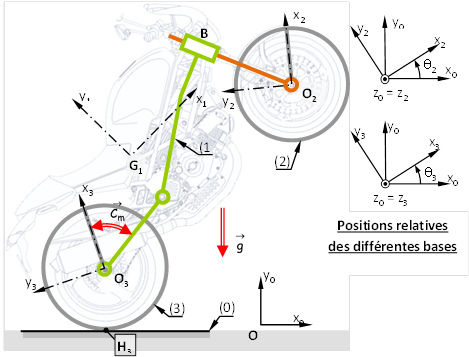
\includegraphics[width=\linewidth]{fig_01}
\end{center}
\end{minipage}
\hfill
\begin{minipage}[c]{.55\linewidth}
\begin{center}
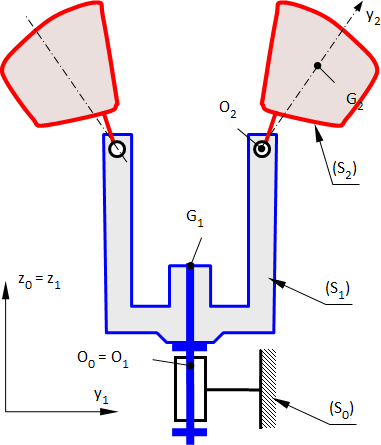
\includegraphics[width=\linewidth]{fig_02}
\end{center}
\end{minipage}
\end{figure*}

\textbf{Remarques :}
\begin{itemize}
\item Entre les pièces (ou les groupes de pièces), on matérialise les liaisons (dont vous connaissez super bien les torseurs).
\item Entre certaines pièces (ou groupes de pièces), il peut exister des actions mécaniques extérieures qui agissent << en positif >> sur une des pièces et << en négatif >> sur l'autre. \textbf{C'est par exemple le cas des moteurs et des vérins}. Il faut bien préciser que l'action mécanique agit sur les deux pièces.
\item Les actions strictement extérieures (comme la pesanteur) ne sont pas en interactions entre deux pièces.
\end{itemize}


\subsection{Isoler les solides soumis à 2 glisseurs}

On commence toujours, \large{toujours}, \Large{toujours}, \LARGE{toujours}, \huge{toujours} \normalsize par isoler les ensembles soumis à 2 glisseurs... Mais cela vous le saviez :). Cependant, en dynamique ce cas est rare. On peut le rencontrer, dans le cas des problèmes plans, lorsque la masse d'un solide est négligée.


\subsection{Cas des chaînes ouvertes}

\begin{marginfigure}
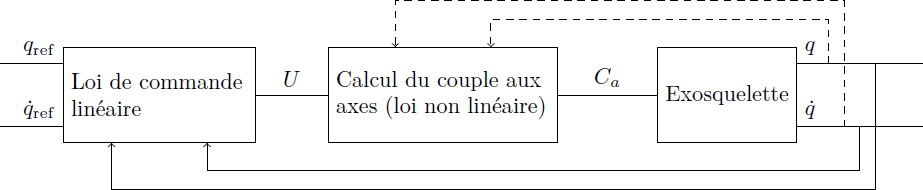
\includegraphics[width=\linewidth]{fig_06}
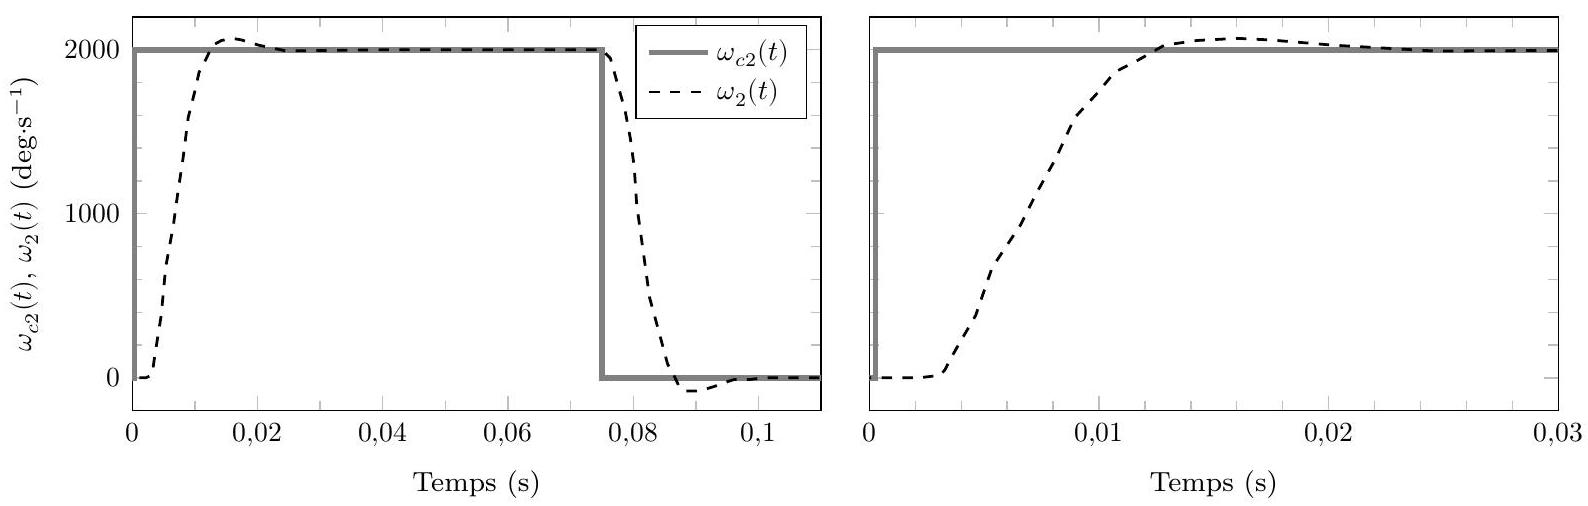
\includegraphics[width=\linewidth]{fig_07}
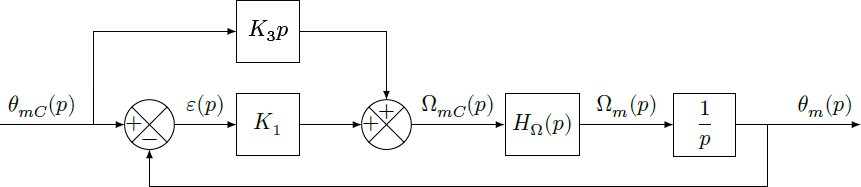
\includegraphics[width=\linewidth]{fig_08}
\end{marginfigure}

C'est le cas le plus rencontré en dynamique. 

On commence par isoler le bout de chaîne. Puis on réalise le théorème correspondant à a mobilité de cet ensemble et on poursuit le raisonnement. 



Ainsi, pour la figure ci-contre :
\begin{enumerate}
\item pour obtenir $C_{m3}$, on isole 4 et on fait un théroème du moment dynamique en $C$ en projection sur $\vz{}$;
\item pour obtenir $C_{m2}$, on isole \{4+3\} et on fait un théroème du moment dynamique en $B$ en projection sur $\vy{}$;
\item pour obtenir $F_{v}$, on isole \{4+3+2\} et on fait un théroème de la résultante dynamique en projection sur $\vx{}$.
\end{enumerate}


\subsection{Cas des chaînes fermées}

Ce cas n'est pas le plus fréquent. Lorsqu'on désire obtenir la loi de mouvement d'une chaîne fermée, il est généralement plus rapide d'uiliser le théorème de l'énergie cinétique que nous aborderons plus tard. 

Pous les chaînes fermées, on va réaliser une coupure << fictive >> dans le système et reprendre la méthode précédente. 

L'objectif et que toutes les équations dynamiques fassent apparaître les inconunes statiques d'une seule et même liaisons. Cela permettra finalement de disposer d'assez d'équations pour supprimer ces inconnues de liaisons.

\begin{marginfigure}
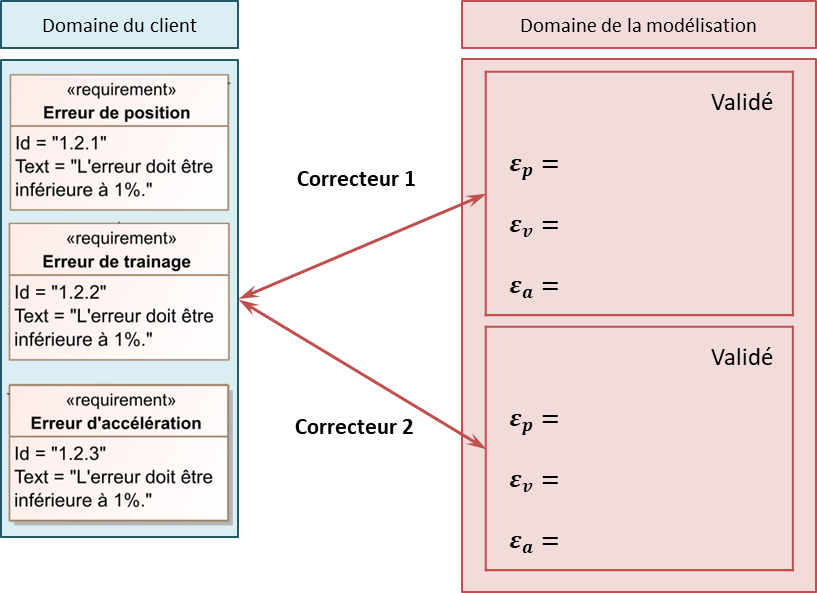
\includegraphics[width=\linewidth]{fig_09}
\end{marginfigure}

Pour l'exemple ci-contre : 
\begin{enumerate}
\item on isole 4 et on réalise un théorème de la résultante dynamique en projection sur $\vy{}$;
\item on isole 3 et on réalise un théorème du moment dynamique en $B$ en projection sur $\vz{}$;
\item on isole \{2+3\} et on réalise un théorème du moment dynamique en $A$ en projection sur $\vz{}$.
\end{enumerate}



\subsection{Cas des véhicules}
Dans les cas des véhicules, l'application du PFD permet de déterminer 
\begin{itemize}
\item les conditions de dérapages en ligne droite ou en virage;
\item les conditions de basculent en ligne droite ou en virage.
\end{itemize}



\subsection{Il y a plus qu'à ...}
\subsubsection{Produit mixte}
Petite remarque pour finir : le produit mixte. Lorsqu'on applique un TMS suivant une direction, le produit mixte peut être un bon outil :
$\vectm{B}{1}{2}\cdot \vect{z} = \left( \vectm{A}{1}{2} + \vect{BA}\wedge \vectf{1}{2}\right)\cdot \vect{z}$
$=  \vectm{A}{1}{2}\cdot \vect{z} + \left(\vect{BA}\wedge \vectf{1}{2}\right)\cdot \vect{z}$...
et $\left(\vect{u} \wedge \vect{v}\right) \cdot \vect{z}= \left(\vect{v} \wedge \vect{z}\right) \cdot \vect{u}= \left(\vect{z} \wedge \vect{u}\right) \cdot \vect{v}$.

\subsubsection{Projection de la dérivée et dérivée de la projection...}